\documentclass[a4paper,10pt]{article}
\usepackage[utf8]{inputenc}
\usepackage{graphicx}       % Pictures
\graphicspath{{./img/}} % Path
\usepackage{fullpage}      % Margens
\usepackage{indentfirst}   % Autoidentar

\begin{document}

\thispagestyle{empty}
\begin{center}

	
\includegraphics[width=5cm]{img/logo2.png}
		
	\vspace*{4cm}
		
	{\Large \bf Decodificação de instruções \textit{Thumb}}
		
	\vspace*{4.5cm}
		
	{\Large \bf Nome: João Pedro Oliveira Santiago	\,\,  Matricula: 404736}
		
		
	\vspace*{9.5cm}
		
	{\Large \bf Quixadá-CE\\
	2019}

\end{center}
	
\setcounter{page}{0}
	\section*{Compilação e execução do programa}
	
	O código fonte do programa consiste em quatro arquivos, são eles \textit{decode.cpp, decode.hpp, makefile e in.s}.
	
	O \textit{Makefile} está configurado para compilar o programa e gerar binário que pode ser executado, chamado de \textit{decode.bin}. Para compilar, basta digitar \textit{make}.
	
	O processo de como compilar está ilustrado abaixo:
	\begin{center}
		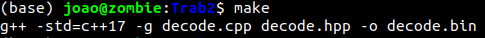
\includegraphics[width=10cm]{img/arq1.png}
	\end{center}
	
	Com o binário gerado, podemos digitar \textit{./decode.bin} para a execução do programa.
	
	Podemos ver o binário gerado pela compilação digitando o comando \textit{ls}.
	
	\begin{center}
		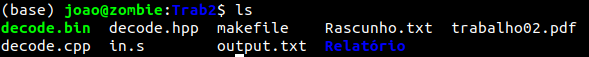
\includegraphics[width=10cm]{img/arq2.png}
	\end{center}	
	
	Executando o programa, o é gerado um arquivo chamado \textit{output.txt}, com as instruções decodificadas. E podemos visualizar seu conteúdo digitando o comando \textit{cat output.txt}.
	\begin{center}
		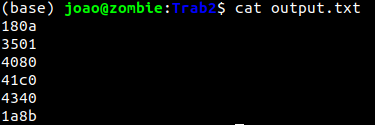
\includegraphics[width=10cm]{img/arq3.png}
	\end{center}
	
	Caso queira, pode limpar o binário gerado, juntamente com o arquivo de saída. Para tal basta digitar \textit{make clean}.
	
	\section*{Decodificador de instruções}
	
	
\end{document}